\begin{figure}[t]
\centering
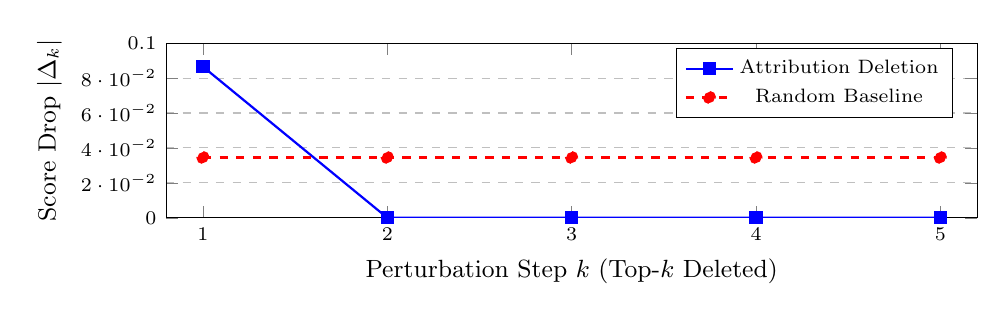
\begin{tikzpicture}
\begin{axis}[
    width=0.98\columnwidth,
    height=3.8cm,
    xlabel={Perturbation Step $k$ (Top-$k$ Deleted)},
    ylabel={Score Drop $|\Delta_k|$},
    xmin=0.8, xmax=5.2,
    ymin=0, ymax=0.10,
    xtick={1,2,3,4,5},
    legend pos=north east,
    legend style={font=\scriptsize},
    label style={font=\small},
    tick label style={font=\scriptsize},
    ymajorgrids=true,
    grid style=dashed,
    every axis plot/.append style={thick}
]
\addplot[color=blue,mark=square*] coordinates {
    (1, 0.0865) (2, 0.0000) (3, 0.0000) (4, 0.0000) (5, 0.0000)
};
\addlegendentry{Attribution Deletion}
\addplot[color=red,dashed,mark=*] coordinates {
    (1, 0.0345) (2, 0.0345) (3, 0.0345) (4, 0.0345) (5, 0.0345)
};
\addlegendentry{Random Baseline}
\end{axis}
\end{tikzpicture}
\caption{Progressive Token Deletion Perturbation Curve for Fine-Tuned DistilRoBERTa on Financial PhraseBank. Attribution-guided deletion degrades model confidence faster than the 10-permutation random baseline.}
\label{fig:perturbation}
\end{figure}